\documentclass[12pt]{article}

\usepackage{amssymb}
\usepackage{amsmath}
\DeclareMathOperator*{\argmax}{arg\,max}
\usepackage{indentfirst}
%\usepackage[T1]{fontenc} % Use 8-bit encoding that has 256 glyphs
\linespread{1.5} % Line spacing - Palatino needs more space between lines

\usepackage[hmarginratio=4:3, top=20mm, left=30mm, columnsep=20pt]{geometry} % Document margins
\usepackage[hang, small,labelfont=bf,up,textfont=it,up]{caption} % Custom captions under/above floats in tables or figures

\usepackage{enumitem} % Customized lists
\setlist[itemize]{noitemsep} % Make itemize lists more compact

\usepackage{abstract} % Allows abstract customization
\renewcommand{\abstractnamefont}{\normalfont\bfseries} % Set the "Abstract" text to bold
\renewcommand{\abstracttextfont}{\normalfont\small\itshape} % Set the abstract itself to small italic text

\usepackage{titlesec} % Allows customization of titles
\renewcommand\thesection{\Roman{section}} % Roman numerals for the sections
\renewcommand\thesubsection{\roman{subsection}} % roman numerals for subsections
\titleformat{\section}[block]{\large\scshape\centering}{\thesection.}{1em}{} % Change the look of the section titles
\titleformat{\subsection}[block]{\large}{\thesubsection.}{1em}{} % Change the look of the section titles

\usepackage{fancyhdr} % Headers and footers
\pagestyle{fancy} % All pages have headers and footers
\fancyhead{} % Blank out the default header
\fancyfoot{} % Blank out the default footer
% \fancyhead[C]{Running title $\bullet$ May 2016 $\bullet$ Vol. XXI, No. 1} % Custom header text
\fancyfoot[RO,LE]{\thepage} % Custom footer text

\usepackage{titling} % Customizing the title section

\usepackage{hyperref} % For hyperlinks in the PDF

\usepackage{graphicx}

%----------------------------------------------------------------------------------------
%	TITLE SECTION
%----------------------------------------------------------------------------------------

\setlength{\droptitle}{-4\baselineskip} % Move the title up

\pretitle{\begin{center}\Large\bfseries} % Article title formatting
\posttitle{\end{center}} % Article title closing formatting
\title{Optimal couponing in retail: a bayesian approach} % Article title
\author{%
\textsc{Sarapulov G. V.} \\ % Your name
%\textsc{John Smith}\thanks{A thank you or further information} \\[1ex] % Your name
\normalsize Saint-Petersburg State University \\ % Your institution
\normalsize Faculty of mathematics and mechanics \\ % Your institution
\normalsize \href{mailto:g-eos@yandex.ru}{g-eos@yandex.ru} % Your email address
}
\date{\today} % Leave empty to omit a date
\renewcommand{\maketitlehookd}{%
\begin{abstract}
%\noindent \blindtext % Dummy abstract text - replace \blindtext with your abstract text
A problem of optimal couponing in retail is addressed by applying naive bayes classifiers to estimate a probability of item purchase with and without discount and choosing the available coupon with maximum difference between these estimates. It is experimentally shown that proposed methodology is able to significantly increase the conversion rate while maintaining high interpretability and scalability.
\end{abstract}
}

\begin{document}
\maketitle


\section{Introduction}
Growing interest of business in using big data and machine learning leads to new decisions in different known issues. Personalized discount strategy is one of such tasks. Product retail, unlike other fields where recommender systems are actively used (streaming services, e-commerce, search engines etc.), has several traits that make standard approaches unapplicable. Firstly, explicit ratings of items are unavailable due to difficulties of collecting them, so only transactional data is available to inference user preferences. Secondly, it is not enough to recommend an item to a customer to stimulate purchase: customers are already aware of available items, have stable tastes and tend to repeatedly buy those they liked before, and discounts are usually used to increase sales. So a task of recommending an item naturally transforms to a task of offering the most relevant discount coupon. \par

In this article we propose an approach to couponing based on comparing the probabilities of item purchases with and without discount and choosing the coupon with maximum difference between these probabilities. This method is highly interpretable (we offer a discount that increases the probability of item purchase most of all) and computationally effective, as it is based on naive assumptions of features conditional indepedence. Despite its simplicity, described approach is able to generate personalized offers with high conversion rate, as was shown experimentally, thus being particularly useful instrument for marketing tasks. \par

The article is structured as follows. Section II provides notation and formal definition of the problem. Section III presents a detailed description of optimal coupon choice based on purchase data. Experimental results are summarized in section IV. \par

\section{Formal problem definition}
Here we introduce a notation used further:
\begin{itemize}
\item $U$ - a set of customers
\item $I$ - a set of items
\item $C = \{(i, d)\}$ - a set of available coupons (pairs item-discount)
\item $R = \{(t, u, i)\}$ - a set of transactions described as (date, cistomer-item)
\item $D = \{(t, u, i, d, s)\}$ - a set of issued coupons described as (date, customer, item, discount, conversion flag)
\end{itemize}

Let's also denote $\mathbf{x_u} = \{x_{u1}, ..., x_{uN}\} \in \mathbf{X}$  as feature vector of customer $u$, formed on transaction history $R$ for last $T$ days, where $x_{ui} = 1$, if customer $u$ purchased item $i$, and $x_{ui} = 0$ otherwise. Analogously $\mathbf{y_u} = \{y_{u1}, ..., y_{uN}\} \in \mathbf{Y}$ denotes the next transaction of a customer $u$. Each issued coupon from $D$ is represented by vector $\mathbf{z_u} = \{z_{u1}, ..., z_{uM}\} \in \mathbf{Z}$, where $z_{uc} = 1$, if customer $u$ used coupon $c$. \par

Our aim is to provide a customer with personalized discount that would most likely lead to item purchase, while no being excessive: if the customer is likely to buy an item even without discount, then coupon will only lead to margin decrease. \par
 
Formally, based on previous transactions $R$ and earlier issued coupons $D$ for each customer $u \in U$ we chooce an item $i$ with discount $d$, i.e. coupon $c = (i, d)$ from a set of available coupons $C$, such that the difference between probabilities of this item purchase with coupon $c = (i, d)$ and without discount is maximized:
\begin{equation}
c_u^* = \argmax_{c \in C, c = (i, d)} P(z_{uc} = 1 | \mathbf{x_u}) - P(y_{ui} = 1 | \mathbf{x_u})
\end{equation}
\par

\section{Proposed approach}

To estimate these probabilities, two probabilistic models are needed. First one will be used to predict item purchases in the next transaction depending on content of all previous transactions of customer for period $T$. Second model will estimate probabilities of coupons conversion based on the same data as first model uses. After we obtain the probabilities of item $i$ purchase and all the corresponding coupons conversion, i.e. coupons that provide some discount $d$ for item $i$, we will be able to choose an optimal coupon for each customer. \par

We will use "naive" assumption that Bernoulli random variables $x_{ui}$ are independent given $\mathbf{y_u}$:
\begin{equation}
P(x_{ui} | x_{uj}, \mathbf{y_u}) = P(x_{ui} | \mathbf{y_u}), i \ne j
\end{equation}
For each item $i \in I$ we fit a naive bayes classifier $f_i: \mathbf{X} \rightarrow y_i$ to estimate a probability of item $i$ purchase given the content of previous purchases:
\begin{equation}
P(y_i = 1 | \mathbf{x_u}) = \frac{P(y_i = 1) \cdot P(\mathbf{x_u} | y_i = 1)}{P(\mathbf{x_u})} = \frac{P(y_i = 1) \cdot \prod_{j=1}^N P(x_{uj} | y_i = 1)}{\prod_{j=1}^N P(x_{uj})}
\end{equation}
Similarly for each coupon $c \in C$ we fit a classifier $f_c: \mathbf{X} \rightarrow z_c$ to estimate the probability of coupon conversion:
\begin{equation}
P(z_c = 1 | \mathbf{x_u}) = \frac{P(z_c = 1) \cdot P(\mathbf{x_u} | z_c = 1)}{P(\mathbf{x_u})} = \frac{P(z_c = 1) \cdot \prod_{j=1}^N P(x_{uj} | z_c = 1)}{\prod_{j=1}^N P(x_{uj})}
\end{equation}
Optimal coupon is then obtained with the following formula:
\begin{equation}
c_u^* = \argmax_{c \in C, c = (i, d)} f_c(\mathbf{x_u}) - f_i(\mathbf{x_u})
\end{equation}
\par

\section{Experimental results}
The described approach was tested on product chain stores. We used transactions of 30-days period before coupon issue to fit our models. The experiment was aimed to increase conversion rate, that, in turn, can help increase other marketing indicators (in particular, average order sum and churn rate). \par

\begin{figure}
  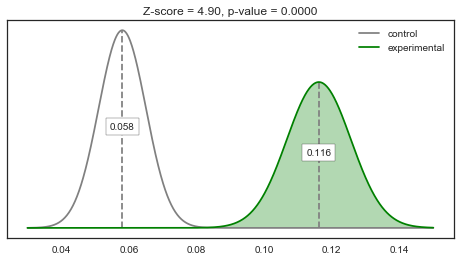
\includegraphics[width=\linewidth]{b.jpg}
  \caption{Conversion rate in experimental groups}
  \label{fig:exp}
\end{figure}

We used a split test to evaluate the conversion rate difference between experimental group, who got coupons provided by proposed method, and control group, who got regular coupons formed by existing recommender system amplified with business logic rules. Picture  \ref{fig:exp} represents conversion rates in customer groups. Fischer's Z-test shows that conversion rate of experimental group (11.6\%) is higher than conversion rate of control group (5.8\%) with a confidence level of 99\%. \par

Obtained result is provided by relatively simple probabilistic models and can be improved, though even in current configuration it achieved better result in terms of conversion rate than masive business logic exploited earlier, that took a great amount of resources to be developed and is not hard to maintain. A described approach is flexible to use it for optimization of different metrics. Another advantage is the ability to incrementally update models with new data to adapt to changing internal (pricing policy, mass promotions) and external (seasonality, competition) factors. \par

\begin{thebibliography}{99} % Bibliography - this is intentionally simple in this template
\bibitem{}
Yifan Hu , Yehuda Koren , Chris Volinsky, Collaborative Filtering for Implicit Feedback Datasets, Proceedings of the 2008 Eighth IEEE International Conference on Data Mining, p.263-272, December 15-19, 2008

\bibitem{}
Ruslan Salakhutdinov, Andriy Mnih, Geoffrey Hinton, Restricted Boltzmann machines for collaborative filtering, Proceedings of the 24th international conference on Machine learning, p.791-798, June 20-24, 2007, Corvalis, Oregon, USA

\bibitem{}
Evangelia Christakopoulou , George Karypis, Local Item-Item Models For Top-N Recommendation, Proceedings of the 10th ACM Conference on Recommender Systems, September 15-19, 2016, Boston, Massachusetts, USA  
\bibitem{}
Christopher M. Bishop, Pattern Recognition and Machine Learning (Information Science and Statistics), Springer-Verlag New York, Inc., Secaucus, NJ, 2006

\end{thebibliography}

\end{document}
